\section{Auswertung}
\label{sec:Auswertung}

Zunächst muss die Apperatur vermessen werden.
Die Messergebnisse werden in Tabelle \ref{tab:1} und \ref{tab:2} präsentiert.

\begin{table}[H]
  \centering
  \caption{Radius des Torsionsfadens}
  \label{tab:1}
  \sisetup{table-format=1.2}
  \begin{tabular}{c}
    \toprule
    {$r [\si{\micro\second}]$}\\
    \midrule
    \input{build/radius_tabelle.tex}
    \bottomrule
  \end{tabular}
\end{table}

\begin{table}[H]
  \centering
  \caption{Länge des Torsionsfadens oberhalb/unterhalb des Spiegels}
  \label{tab:2}
  \sisetup{table-format=1.2}
  \begin{tabular}{c c}
    \toprule
    {$L1 [\si{\centi\metre}]$} & {$L2 [\si{\centi\metre}]$}\\
    \midrule
    \input{build/laengen_tabelle.tex}
    \bottomrule
  \end{tabular}
\end{table}

















%\begin{figure}
%  \centering
%  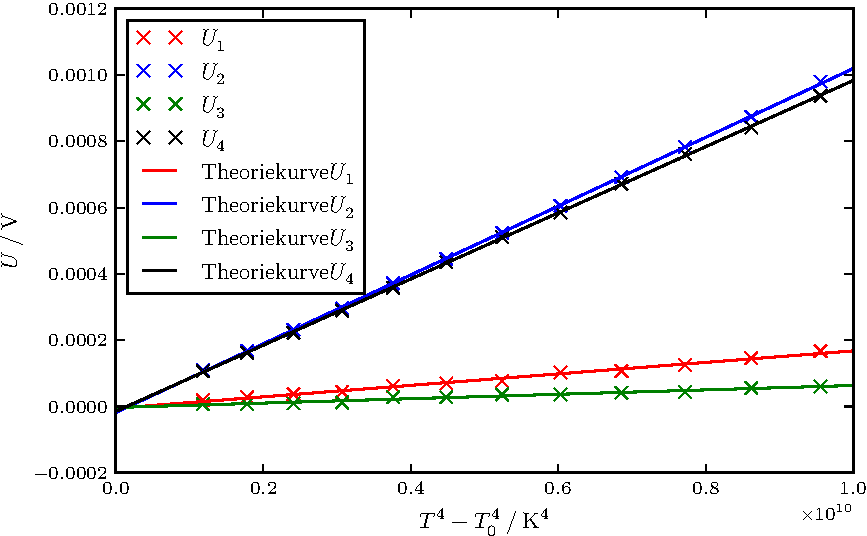
\includegraphics{plot.pdf}
%  \caption{Plot.}
%  \label{fig:plot}
%\end{figure}
%
%\begin{table}
%  \centering
%  \caption{Beispieltabelle}
%  \label{tab:tabelle_beispiel}
%  \sisetup{table-format=1.2}
%  \begin{tabular}{c c}
%    \toprule
%    {$a [\si{\second}]$} & {$b [\si{\kelvin}]$}\\
%    \midrule
%    1.0000  & 11.00 \\
2.0000  & 12.00 \\
3.0000  & 13.00 \\
4.0000  & 14.00 \\
5.0000  & 15.00 \\
6.0000  & 16.00 \\
7.0000  & 17.00 \\
8.0000  & 18.00 \\
9.0000  & 19.00 \\
10.0000 & 20.00 \\

%    \bottomrule
%  \end{tabular}
%\end{table}
%
%Es ergibt sich
%\begin{align}
%  a &= (0 \pm 0) ~ \si{\joule\per\kelvin\per\gram}
 \\
%\end{align}
